% Part: sets-functions-relations
% Chapter: relations
% Section: graphs

\documentclass[../../../include/open-logic-section]{subfiles}

\begin{document}

\olfileid{sfr}{rel}{grp}
\olsection{গ্রাফ}

একটি \emph{গ্রাফ} হল এমন চিত্র যাতে বিন্দুগুলি---যাদের ``নোড'' বা ``শীর্ষ'' বলা হয়---প্রান্ত দিয়ে যুক্ত থাকে। বিচ্ছিন্ন গণিত ও কম্পিউটার বিজ্ঞানে গ্রাফ সর্বত্র ব্যবহৃত হয়। বিভিন্ন ধরনের নেটওয়ার্কের মতো মূর্ত বিষয় থেকে শুরু করে সিদ্ধান্তের সম্ভাব্য ফলাফলের মতো বিমূর্ত কাঠামো পর্যন্ত নানা সম্পর্ক ও কাঠামো প্রকাশ করতে এবং চিত্রের সাহায্যে বুঝতে এগুলি অত্যন্ত কার্যকর। সাহিত্যে বিভিন্ন ধরনের গ্রাফ দেখা যায়; যেমন, প্রান্তের দিকনির্দেশ আছে কি না, প্রান্তে লেবেল আছে কি না, কোনো নোড থেকে সেই নোডেই প্রান্ত থাকতে পারে কি না, একই নোডগুলির মধ্যে একাধিক প্রান্ত থাকতে পারে কি না, ইত্যাদি অনুসারে তারা ভিন্ন হয়। \emph{নির্দেশিত গ্রাফের} সঙ্গে সম্পর্কের একটি বিশেষ যোগ আছে।

\begin{defn}[নির্দেশিত গ্রাফ]
একটি \emph{নির্দেশিত গ্রাফ} $G = \tuple{V, E}$ হল \emph{শীর্ষের} সেট~$V$ এবং \emph{প্রান্তের} সেট~$E \subseteq V^2$ নিয়ে গঠিত।
\end{defn}

\begin{explain}
আমাদের সংজ্ঞা অনুসারে, একটি গ্রাফ আসলে একটি সেট এবং সেই সেটের উপর একটি সম্পর্ক নিয়ে গঠিত। অবশ্য গ্রাফের কথা বললে তার একটি চিত্র প্রত্যাশা করাই স্বাভাবিক: আমরা দুটি শীর্ষ~$v_1$ ও $v_2$-কে একটি তির দিয়ে যুক্ত করে গ্রাফ আঁকতে পারি যদি এবং কেবল যদি $\tuple{v_1, v_2} \in E$ হয়। একটি সম্পর্ককে একা বিবেচনা করা এবং একটি গ্রাফের মধ্যে একমাত্র পার্থক্য হল, গ্রাফে শীর্ষের সেট নির্দিষ্ট করা থাকে; অর্থাৎ গ্রাফে বিচ্ছিন্ন শীর্ষ থাকতে পারে। তবে মূল কথা হল, একটি সেট~$X$-এর উপর প্রত্যেক সম্পর্ক~$R$-কে নির্দেশিত গ্রাফ $\tuple{X, R}$ হিসেবে দেখা যায়; এবং বিপরীতভাবে, একটি নির্দেশিত গ্রাফ~$\tuple{V, E}$-কে $V$ সেটটি স্পষ্টভাবে নির্দিষ্ট করা আছে এমন সম্পর্ক $E \subseteq V^2$ হিসেবে দেখা যায়।
\end{explain}

\begin{ex}
$V = \{1, 2, 3, 4\}$ এবং $E = \{\tuple{1,1}, \allowbreak \tuple{1, 2}, \allowbreak \tuple{1, 3}, \allowbreak \tuple{2, 3}\}$ হলে গ্রাফ $\tuple{V, E}$-এর চিত্র এইরকম:
\begin{align*}
& 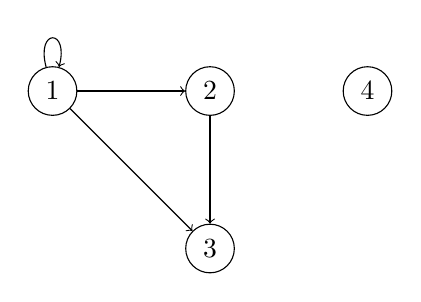
\begin{tikzpicture}[->,node distance=2cm]
  \node[draw,circle] (A) {$1$};
  \node[draw,circle] (B) [right of=A] {$2$};
  \node[draw,circle] (C) [below of=B] {$3$};
  \node[draw,circle] (D) [right of=B] {$4$};
  \draw (A) to [loop above]  (A);
  \draw (A) to  (B);
  \draw (A) to  (C);
  \draw (B) to  (C);
  \end{tikzpicture}
\intertext{এটি $V' = \{1, 2, 3\}$-বিশিষ্ট গ্রাফ $\tuple{V', E}$ থেকে আলাদা; সেই গ্রাফের চিত্র এইরকম:}
& 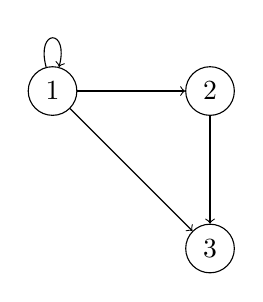
\begin{tikzpicture}[->,node distance=2cm]
  \node[draw,circle] (A) {$1$};
  \node[draw,circle] (B) [right of=A] {$2$};
  \node[draw,circle] (C) [below of=B] {$3$};
  \draw (A) to [loop above]  (A);
  \draw (A) to  (B);
  \draw (A) to  (C);
  \draw (B) to  (C);
  \end{tikzpicture}
\end{align*}
\end{ex}

\begin{prob}
  $\{1, 2, 3, 4\}$ সেটের উপর ছোট-অথবা-সমান সম্পর্ক~$\le$-কে গ্রাফ হিসেবে বিবেচনা করে তার চিত্র আঁকো।
\end{prob}

\end{document}
